\documentclass{article}
\usepackage[utf8]{inputenc}
\usepackage{amsfonts}
\usepackage{algorithm2e}
\usepackage{amsmath}
\usepackage[a4paper]{geometry}
\geometry{hscale=0.8,vscale=0.9,centering}
\usepackage{graphicx}
\usepackage{program}
\usepackage{ulem}
\usepackage{xcolor}
\usepackage{pdfpages}
\usepackage{hyperref}
\newcommand{\subsubsubsection}[1]{\paragraph{#1}\mbox{}\\}
\setcounter{secnumdepth}{4}
\setcounter{tocdepth}{4}
\newcommand{\alinea}{
\textbf{\hspace{8mm}}
}
 \setlength{\parindent}{0pt}
 
\newcommand{\sautligne}{
\textbf{\vspace{5mm}}
}



\title{M1 Info – ARC - LAB4}
\author{Olivier HUREAU - Groupe 3}
\date{25/03/2020}

\begin{document}
\maketitle
\renewcommand{\contentsname}{Table des matières}
\tableofcontents
\newpage

\section{Évaluation de la qualité des tests.}
Les différents types de couverture nous intéréssant sont 
\begin{itemize}
	\item State / Transition coverage : En principe les testbench vérifie que la machine passe dans tout les états. Si nous n'avons pas 100\% de couverture ici c'est qu'il y a un problème.
		\item Branch coverage : Si le teste de couverture remonte des erreurs, il sera alors plus facile de traquer les erreurs de transissions..
	\item Expression coverage : Les expressions influant sur les branchements, ce test de couverture nous permet aussi de vérifier le comportement du robot.

\end{itemize}

Les tests "line coverage" et "statemets coverage" donnent une indication sur la présentation ou l'optimisation du code, ne nous souciants uniquement du bon fonctionnement de notre implémentation, il ne nous sont pas utiles.

Le test Toggle coverage donnant une indication sur la robustesse du l'implémentation. Il est bien trop compliqué et trop long d'analyser les résultats de ce test dans le cadre de nos labs.


\subsection{Première analyse}

\subsubsection{Résultats du test de coverage}

\paragraph{Résultats du test de coverage sur le système entier}

Ci dessous : S est l'architecture System, C1 et C2 les compteurs et R le robots dans le testbench System.
\begin{figure}[!h]
\advance\leftskip+3cm
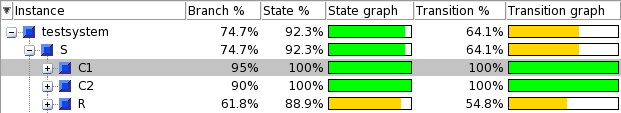
\includegraphics[scale=0.70]{PremiereAnalyse/Coverage.PNG}
\caption{Résultats de couverture Branch, State et Transition sur le système entier}
\end{figure}

Le graph de couverture du robot dans le testbench system

\begin{figure}[!h]
\advance\leftskip+3cm
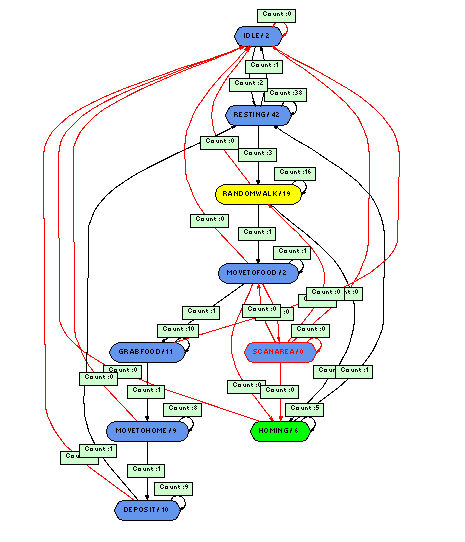
\includegraphics[scale=0.80]{PremiereAnalyse/graph.PNG}
\caption{Graph de couverture d'état sur le système entier}
\end{figure}

\paragraph{Résultats du test de coverage sur le robot}

Ci dessous : S est l'architecture System, C1 et C2 les compteurs et R le robots dans le testbench System.
\begin{figure}[!h]
\advance\leftskip+3cm
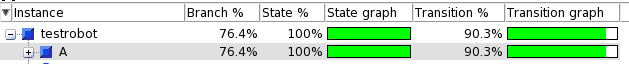
\includegraphics[scale=0.70]{PremiereAnalyse/coverRobot.PNG}
\caption{Résultats de couverture Branch, State et Transition sur le robot}
\end{figure}

Le graph de couverture du robot dans le testbench system

\begin{figure}[!h]
\advance\leftskip+3cm
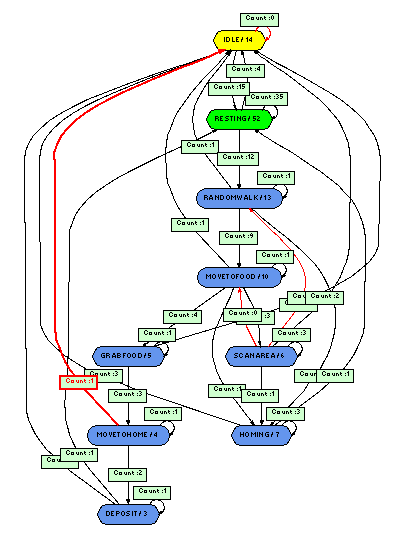
\includegraphics[scale=0.80]{PremiereAnalyse/graphRobot.PNG}
\caption{Graph de couverture d'état sur le robot}
\label{graphe-robot}
\end{figure}


\paragraph{Interprétation des résultats}
\sautligne

Les tests de couverture sont très probant (87\% pour le système entier). Cependants, on vois que des dans le système entier, l'état SCANAREA n'est jamais atteins bien que les tests de système (se reporter au tableau du précédent lab) avais prévu un chemin pour arriver jusqu'à cet état ainsi que d'utiliser ses transitions. 

L'analyse du robot avec un testbench différent nous donne alors des indications suivantes : certaines transitions ne sont jamais atteintes, l'état SCANAREA est bien accessible pour l'automate. 
\sautligne

Deux hyptohèses se posent alors : Soit le système est mal conçus, soit c'est les testbenchs. Avant de se replonger dans le une éventuelle réécriture des architectures et/ou entité (la couverture des branch pourrons nous aider pour cela). Il faut être certains que c'est les testbenchs qui ne sont pas faux.


\newpage
\subsection{Correction du code après une première analyse}

Après interprétation des résultats, on créer des séquences de signaux qui nous permettrons d'être sur que le testbenchs du robot n'est pas faux.
\sautligne

Grace au graph de couverture (figure \ref{graphe-robot}) il faut tester les transitions suivantes :
\begin{itemize}
\item Reset depuis MOVETOHOME
\item Aller de SCANAREA à MOVETOFOOD (rappel de contraintes de transition : Aboveseartch ='0' \& findfood = '0' \& scantimeup = '1')
\item Aller de SCANAREA à RANDOMWALK (rappel de contraintes de transition : Aboveseartch ='0' \& findfood = '1' )
\end{itemize}


\subsection{Deuxième analyse}


\section{Vérification d'assertions temporelles}

 
\end{document}